% !TeX spellcheck = en_GB
\section{International market entry}

\subsection{Decision for international market entry}

To decide in which country and how we want to export goods we have to consider the following three steps:

\begin{enumerate}
	\item Prioritize countries based on market attractiveness and market risks
	\item Define a business plan for attractive countries to prepare final decision
	\item Define type of market entry
\end{enumerate}

\subsubsection{Market prioritization}

Analyse and score market attractiveness and market risks to distinguish between 1st, 2nd, 3rd and 4th priority markets.

\paragraph{Market attractiveness criteria}
\begin{itemize}
	\tightlist
	\item Size of market
	\item Growth of market
	\item Customer structure
	\item Customer ability to buy
	\item Price situation (for B2B products visiting a fair might be necessary)
	\item Potential partners
	\item Intensity of competition
	\item Our competitive positioning
\end{itemize}

\paragraph{Market risks criteria}
\begin{itemize}
	\tightlist
	\item Political stability
	\item Stability of exchange rate
	\item Transfer risk (e.g. customs)
	\item Operating formalities
	\item Risk of expropriation
	\item Intercultural risk
	\item Internal risks
\end{itemize}

\paragraph{Final analysis}

\begin{enumerate}
	\tightlist
	\item Weight each attractiveness and risk criteria (the sum of weights should be 10 for the attractiveness as well as the risks).
	\item Score each attractiveness and risk with a score between 1-4 (1=bad attractiveness/low risk, 4=very heigh attractiveness/very high risk).
	\item Calculate total risk and attractiveness and prioritise the target country according to the matrix shown in \autoref{fig:market-prioritation}.
\end{enumerate}

\begin{figure}[H]
	\centering
	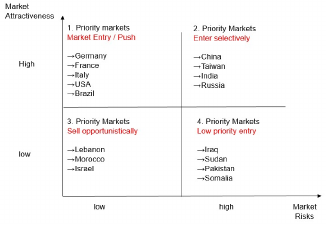
\includegraphics[width=0.7\textwidth]{figures/marketPrioritization.png}
	\caption{Market prioritization matrix}
	\label{fig:market-prioritation}
\end{figure}

\subsubsection{Define a business plan}

Do the following steps in order to create a business plan:

\begin{enumerate}
	\tightlist
	\item Analysis
	\begin{itemize}
		\tightlist
		\item Environment
		\item Cultural challenges
		\item Competition
		\item Company analysis
		\item Customers
		\item Quantitative analysis
	\end{itemize}
	\item SWOT
	\begin{description}
		\tightlist
		\item[Strengths] characteristics of the business or project that give it an advantage over others.
		\item [Weaknesses] characteristics of the business that place the business or project at a disadvantage relative to others.
		\item[Opportunities] elements in the environment that the business or project could exploit to its advantage.
		\item[Threats] elements in the environment that could cause trouble for the business or project.
	\end{description}
	\item Market entry strategy
	\begin{itemize}
		\tightlist
		\item Market segments and customers
		\item Positioning
	\end{itemize}
	\item Marketing mix
	\begin{itemize}
		\tightlist
		\item Product
		\item Price
		\item Promotion
		\item Place
	\end{itemize}
	\item Business case
	\begin{itemize}
		\tightlist
		\item Risk analysis
	\end{itemize}
	\item Proposal/Action plan
\end{enumerate}

\subsection{Types of market entry}

\begin{figure}[H]
	\centering
	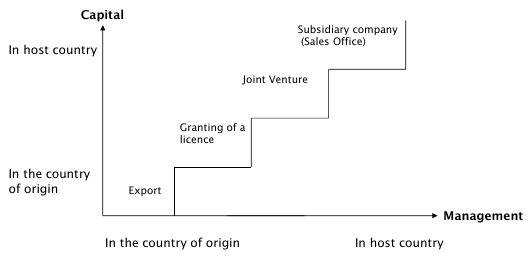
\includegraphics[width=0.7\textwidth]{figures/typesMarketEntry.png}
	\caption{Overview of different types of market entry}
\end{figure}

\subsubsection{Export}
Export means the selling of goods outside the country of manufacture. There are further subcategories of Export:

\begin{description}
	\tightlist
	\item[Indirect export] Collaboration with domestic partners.
	\item[Direct export] Export division, authorised representatives for field work, independent sales agents in foreign countries.
\end{description}

\subsubsection{Licence}
Domestic licensor permits foreign licensee the use of legally protected know-how against fee for a specific territory and a specific period.

\subsubsection{Joint ventures/alliances}
Joint ventures are the foundation of a new trans-national joint venture company where both partner remain legally and economically independent. This results in joint management and risk sharing. In the context of export the \textbf{swiss partner} with \mbox{technological/product} know-how and the \textbf{partner in target country} with market know-how.

\paragraph{Problems} \mbox{}\\
The following problems often arise in joint ventures:

\begin{itemize}
	\tightlist
	\item Objectives are not 100\% clear and communicated to everyone involved
	\item There is an imbalance in levels of expertise, investment or assets brought into the venture by the different partners.
	\item Different cultures and management styles result in poor integration and cooperaion.
	\item The partners don't provide enough leadership and support in the early stages.
\end{itemize}

\paragraph{Why joint ventures often fail}

\begin{itemize}
	\tightlist
	\item Small business owners should not engage in joint ventures without adequate 	planning and strategy.
	\item They cannot afford to, since the ultimate goal of joint ventures is the same as it is for any type of business operation: to make a profit.
	\item Experience dictates that both parties in a joint venture should know exactly 	what they wish to derive from their partnership.
	\item There must be an agreement before the partnership becomes a reality. There must also be a firm commitment on the part of each member to the project and to one another.
	\item One of the leading causes for the failure of joint ventures is that some participants do not reveal their true business agendas, or mislead their partners about their ability to uphold their agreed-upon responsibilities.
	\item Many small business consultants counsel clients to approach joint ventures cautiously. They acknowledge that such partnerships can be most valuable in nourishing a company's growth and stability, but also point out that smaller businesses usually have far less margin for error than do multinational corporations, or even mid-sized companies.
\end{itemize}

\subsubsection{Subsidiary company}
A subsidiary company is a legally independent company in the target country. Instead of establishing a whole company one can also start with a simple sales office.

When talking of subsidiary companies two different types exist:

\begin{description}
	\tightlist
	\item[Brownfield] hen a company purchases an existing production facility to launch a new activity in a target country.
	\item[Greenfield] Start up from scratch of own business in target country.
\end{description}

\subsubsection{Development of market entry}
Market entry modes can change its form over time. See \autoref{fig:development-marketentry} for an example.
\begin{figure}[H]
	\centering
	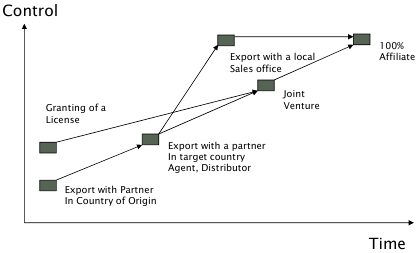
\includegraphics[width=0.7\textwidth]{figures/developmentMarketEntry.png}
	\caption{Development of a market entry}
	\label{fig:development-marketentry}
\end{figure}

\subsubsection{Comparison}
\begin{figure}[H]
	\centering
	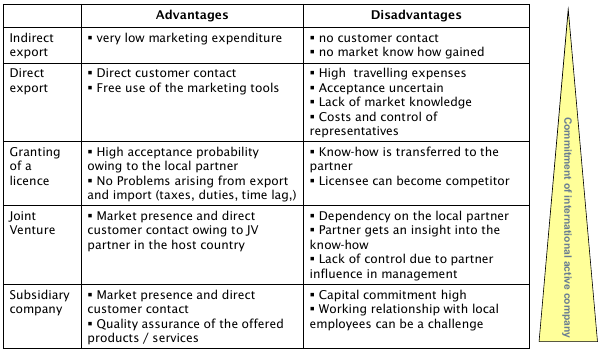
\includegraphics[width=0.9\textwidth]{figures/comparisonMarketEntry.png}
	\caption{Comparison of different market entry modes}
\end{figure}

\subsection{Partner}

\subsubsection{How to select}

\begin{itemize}
	\tightlist
	\item Ask potential customers
	\item Check the partner for references
	\item How good is their distribution network?
	\item You should be a big company for this partner (The partner should be interested in your revenue)
	\item Can they do the service for the products?
	\item Has the partner contact to the industry?
\end{itemize}

\subsubsection{Control}

An important factor when dealing with partners is the controlling of them. You should only pay them for activities performed. A fixed monthly payment is not recommended.

\subsection{Exported product}
\begin{figure}[H]
	\centering
	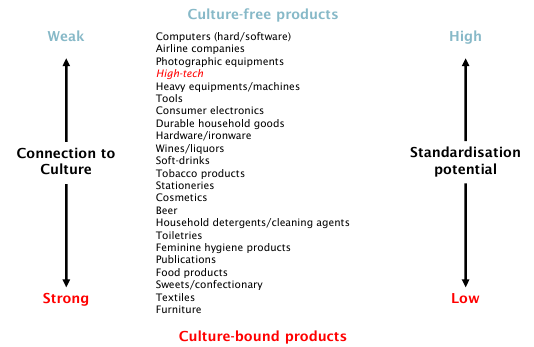
\includegraphics[width=0.9\textwidth]{figures/cultureProduct.png}
	\caption{Culture free and culture bound product}
\end{figure}

Examples:
\begin{description}
	\tightlist
	\item[Culture free product] ABB transformers
	\item[Culture bound product] Nescafé\\
	Nestlé’s success is based firmly on the concept that “food is a local matter“. Although its products are available in virtually every corner of the world, it does not believe in a standard worldwide taste.
\end{description}

\subsubsection{The three layers of a product}
\begin{figure}[H]
	\centering
	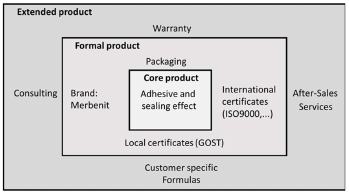
\includegraphics[width=0.6\textwidth]{figures/productLayers.png}
	\caption{Layers of a product}
\end{figure}

\begin{description}
	\tightlist
	\item[Core product] Keep standardized
	\item[Formal product] Follow the laws of the export country.
	\item[Extended product] Used to define USP in export country.
\end{description}

\subsection{Pricing}
 There are two steps of international pricing:
 
 \begin{description}
 	\item[Inside-Out (Cost based)] What is the price to be achieved on the basis of the costs in the target country?\\
 	“Chain of importance:“
 	\begin{enumerate}
 		\tightlist
 		\item Product
 		\item Costs
 		\item Price
 		\item Value
 		\item Customers
 	\end{enumerate}
 	\item[Outside-in (Value based)] Which price can be realized in the target country due to the demand and competition?\\
 	“Chain of importance:“
 	\begin{enumerate}
 		\tightlist
 		\item Customers
 		\item Value
 		\item Price
 		\item Coasts
 		\item Product
 	\end{enumerate}
 \end{description}

\subsubsection{Inside-Out pricing}
When exporting to a foreign country there is often additional cost involved (e.g. translation, transport, duties, fees for distribution partners, ...). These costs must be covered in the export market. There's the danger of price escalation in the export market.

\subsubsection{Outside-in pricing}
To get the price when choosing the outside -in pricing form can be difficult. The following steps might be necessary:

\begin{itemize}
	\tightlist
	\item Make a price study supported by consultant
	\item Visit local trade fairs
	\item Visit potential customers
\end{itemize}

\subsection{Promotion}

There are two different forms of marketing:

\begin{description}
	\tightlist
	\item[Push marketing] \mbox{}\\
	Objective: Distribution partner sells products proactively\\
	Activities: Professionalization and mobilization of distribution partner
	\item[Pull marketing] \mbox{}\\
	Objectives: Customers seek products actively from distribution partner\\
	Activities: Using promotional tools directed towards customers
\end{description}

\subsubsection{Communication barriers}
\begin{figure}[H]
	\centering
	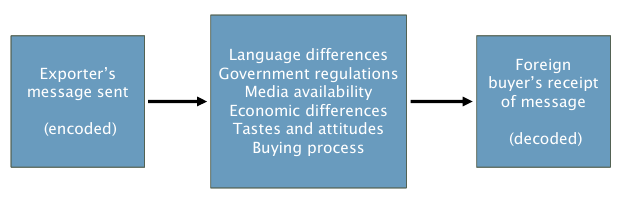
\includegraphics[width=0.8\textwidth]{figures/communicationBarriers.png}
	\caption{Communication barrier}
\end{figure}

\subsubsection{Localized advertisements}
The logos, look and feel should never be adjusted, but the pictures and texts should be localized.
